\documentclass[border=8pt]{standalone}
\usepackage[T1]{fontenc}\usepackage[utf8]{inputenc}
\usepackage{helvet}\renewcommand{\familydefault}{\sfdefault}
\usepackage{tikz,xcolor}
\usetikzlibrary{arrows.meta,positioning,shapes.geometric,shapes.multipart,calc,fit,backgrounds,decorations.markings}
\definecolor{ink}{HTML}{1E1B16}\definecolor{paper}{HTML}{FBF8F2}\definecolor{clay}{HTML}{B5482A}\definecolor{soft}{HTML}{F1E9DA}\definecolor{pine}{HTML}{24402F}
\tikzset{
  every node/.style={font=\small,text=ink},
  >=Stealth, line/.style={draw=ink,line width=0.8pt},
  cls/.style={rectangle split,rectangle split parts=3,draw=ink,line width=0.8pt,fill=soft,align=left,inner xsep=6pt,inner ysep=4pt,
              rectangle split part align={center,left,left},minimum width=3.0cm},
  cls2/.style={rectangle split,rectangle split parts=2,draw=ink,line width=0.8pt,fill=soft,align=left,inner xsep=6pt,inner ysep=4pt,
              rectangle split part align={center,left},minimum width=3.0cm},
  box/.style={rectangle,draw=ink,line width=0.8pt,fill=soft,align=center,inner sep=5pt,minimum height=0.8cm},
  state/.style={rectangle,rounded corners=8pt,draw=ink,line width=0.8pt,fill=soft,align=center,inner sep=6pt,minimum width=2.2cm,minimum height=0.9cm},
  act/.style={rectangle,rounded corners=10pt,draw=ink,line width=0.8pt,fill=soft,align=center,inner sep=5pt,minimum width=2.4cm,minimum height=0.8cm},
  dec/.style={diamond,draw=ink,line width=0.8pt,fill=soft,inner sep=1pt,minimum width=0.9cm,minimum height=0.9cm},
  uc/.style={ellipse,draw=ink,line width=0.8pt,fill=soft,align=center,inner sep=3pt,minimum width=3.2cm,minimum height=1.0cm},
  note/.style={rectangle,draw=ink,line width=0.6pt,fill=yellow!12,align=left,inner sep=4pt,font=\footnotesize},
  lab/.style={font=\footnotesize,fill=paper,inner sep=1.5pt},
  err/.style={},
}
\newcommand{\actor}[3]{% x,y,label
  \draw[line width=0.8pt] (#1,#2+0.55) circle (0.17);
  \draw[line width=0.8pt] (#1,#2+0.38)--(#1,#2-0.15) (#1-0.3,#2+0.22)--(#1+0.3,#2+0.22) (#1,#2-0.15)--(#1-0.25,#2-0.6) (#1,#2-0.15)--(#1+0.25,#2-0.6);
  \node[font=\small] at (#1,#2-0.9) {#3};}
\begin{document}
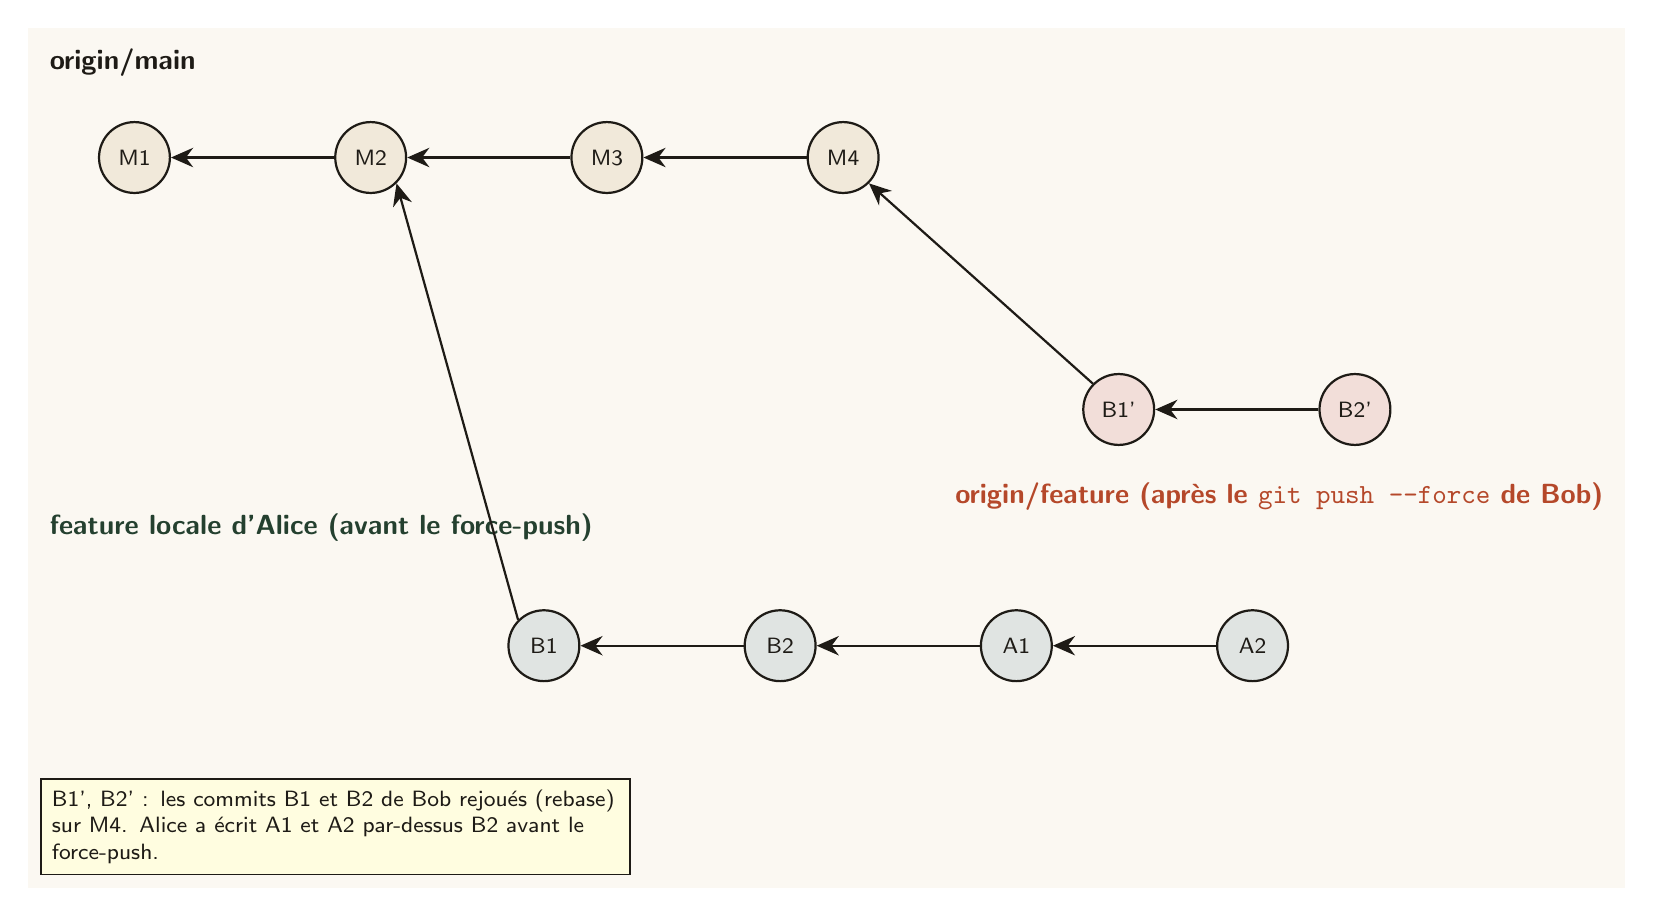
\begin{tikzpicture}[background rectangle/.style={fill=paper},show background rectangle]
\node[anchor=west,font=\bfseries] at (-1.2,4.4) {origin/main};
\node[circle,draw=ink,line width=0.8pt,fill=soft,minimum size=0.9cm,inner sep=0pt] (m0) at (0,3.2) {\footnotesize M1};
\node[circle,draw=ink,line width=0.8pt,fill=soft,minimum size=0.9cm,inner sep=0pt] (m1) at (3,3.2) {\footnotesize M2};
\node[circle,draw=ink,line width=0.8pt,fill=soft,minimum size=0.9cm,inner sep=0pt] (m2) at (6,3.2) {\footnotesize M3};
\node[circle,draw=ink,line width=0.8pt,fill=soft,minimum size=0.9cm,inner sep=0pt] (m3) at (9,3.2) {\footnotesize M4};
\draw[line,-{Stealth[length=8pt,width=7pt]}] (m1.west)--(m0.east);
\draw[line,-{Stealth[length=8pt,width=7pt]}] (m2.west)--(m1.east);
\draw[line,-{Stealth[length=8pt,width=7pt]}] (m3.west)--(m2.east);
\node[anchor=west,font=\bfseries,text=clay] at (10.3,-1.1) {origin/feature (après le \texttt{git push -{}-force} de Bob)};
\node[circle,draw=ink,line width=0.8pt,fill=clay!18,minimum size=0.9cm,inner sep=0pt] (p1) at (12.5,0.0) {\footnotesize B1'};
\node[circle,draw=ink,line width=0.8pt,fill=clay!18,minimum size=0.9cm,inner sep=0pt] (p2) at (15.5,0.0) {\footnotesize B2'};
\draw[line,-{Stealth[length=8pt,width=7pt]}] (p1.north west)--(m3.south east);
\draw[line,-{Stealth[length=8pt,width=7pt]}] (p2.west)--(p1.east);
\node[anchor=west,font=\bfseries,text=pine] at (-1.2,-1.5) {feature locale d'Alice (avant le force-push)};
\node[circle,draw=ink,line width=0.8pt,fill=pine!14,minimum size=0.9cm,inner sep=0pt] (a0) at (5.2,-3.0) {\footnotesize B1};
\node[circle,draw=ink,line width=0.8pt,fill=pine!14,minimum size=0.9cm,inner sep=0pt] (a1) at (8.2,-3.0) {\footnotesize B2};
\node[circle,draw=ink,line width=0.8pt,fill=pine!14,minimum size=0.9cm,inner sep=0pt] (a2) at (11.2,-3.0) {\footnotesize A1};
\node[circle,draw=ink,line width=0.8pt,fill=pine!14,minimum size=0.9cm,inner sep=0pt] (a3) at (14.2,-3.0) {\footnotesize A2};
\draw[line,-{Stealth[length=8pt,width=7pt]}] (a0.north west)--(m1.south east);
\draw[line,-{Stealth[length=8pt,width=7pt]}] (a1.west)--(a0.east);
\draw[line,-{Stealth[length=8pt,width=7pt]}] (a2.west)--(a1.east);
\draw[line,-{Stealth[length=8pt,width=7pt]}] (a3.west)--(a2.east);
\node[note,anchor=west,text width=7.2cm] at (-1.2,-5.3) {B1', B2' : les commits B1 et B2 de Bob rejoués (rebase) sur M4. Alice a écrit A1 et A2 par-dessus B2 avant le force-push.};
\end{tikzpicture}
\end{document}
